\begin{question}
\noindent Shape $A$ and shape $B$ are drawn on the grid below.

\begin{center}
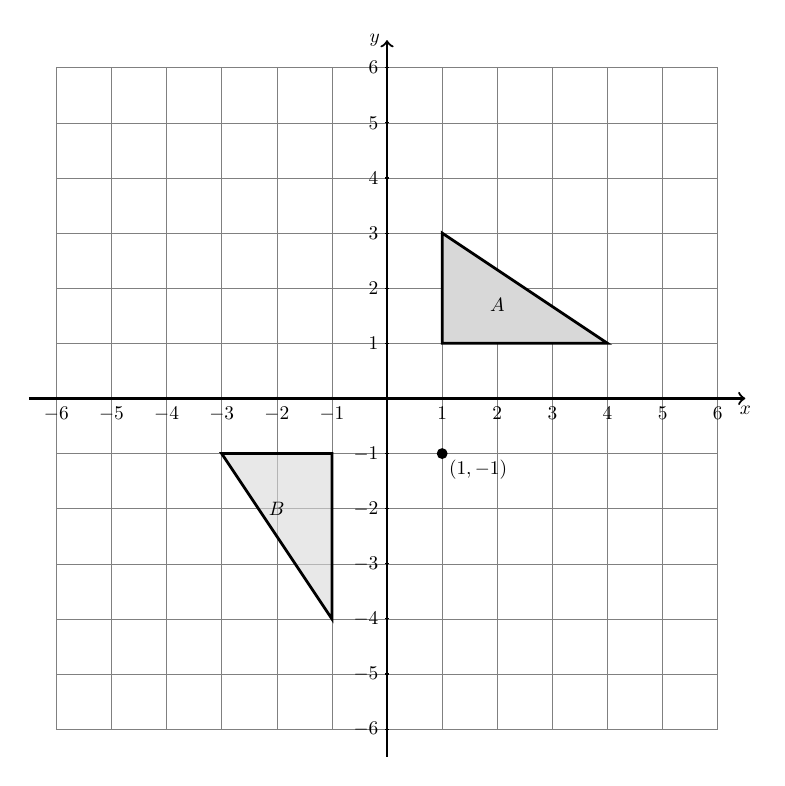
\begin{tikzpicture}[scale=0.7, transform shape]
    % Define colours
    \definecolor{borderColour}{HTML}{000000}
    \definecolor{fillColour}{HTML}{D8D8D8}

    % Define axis scale
    \def\axisLimit{6}

    % Draw grid
    \draw[step=1cm,gray,very thin] (-\axisLimit,-\axisLimit) grid (\axisLimit,\axisLimit);

    % Draw axes
    \draw[thick,->] (-\axisLimit-0.5,0) -- (\axisLimit+0.5,0) node[anchor=north] {$x$};
    \draw[thick,->] (0,-\axisLimit-0.5) -- (0,\axisLimit+0.5) node[anchor=east] {$y$};

    % Label x-axis and y-axis
    \foreach \x in {-6,-5,...,-1,1,2,...,6}
        \draw (\x cm,1pt) -- (\x cm,-1pt) node[anchor=north] {$\x$};
    \foreach \y in {-6,-5,...,-1,1,2,...,6}
        \draw (1pt,\y cm) -- (-1pt,\y cm) node[anchor=east] {$\y$};

    % Shape A: right-angled triangle vertices (1,1), (1,3), (4,1)
    \coordinate (A1) at (1,1);
    \coordinate (A2) at (1,3);
    \coordinate (A3) at (4,1);
    \filldraw[fill=fillColour, draw=borderColour, line width=1pt] (A1) -- (A2) -- (A3) -- cycle;
    \node[below left] at (A1) {};
    \node at (2,1.7) {$A$};

    % Shape B: rotated 90 deg anticlockwise about (1,-1): 
    % (1,1)->(-1,-1)? Let's use centre (1,-1)? We'll define directly with correct coordinates below.
    \coordinate (B1) at (-1,-1);
    \coordinate (B2) at (-3,-1);
    \coordinate (B3) at (-1,-4);
    \filldraw[fill=fillColour, draw=borderColour, line width=1pt, fill opacity=0.6] (B1) -- (B2) -- (B3) -- cycle;
    \node at (-2,-2) {$B$};

    % Mark centre of rotation
    \filldraw[black] (1,-1) circle (2.5pt);
    \node[below right] at (1,-1) {$(1,-1)$};

\end{tikzpicture}
\end{center}

\noindent Describe fully the single transformation that maps shape $A$ onto shape $B$.

\vspace{5cm}

\begin{flushright}
    \answerlines{3}{3}
\end{flushright}
\end{question}
